\icode{E-MI-SI-L3-260627-001}
两个质量均为\(m\)的\(A\)、\(B\)小球用轻杆连接，\(A\)球与固定在斜面上的光滑竖直挡板\(MN\)接触，\(B\)球放在倾角为\(\theta\)的斜面上，\(A\)、\(B\)均处于静止，\(B\)球没有滑动趋势，则\(A\)球对挡板的压力大小为\paren[]

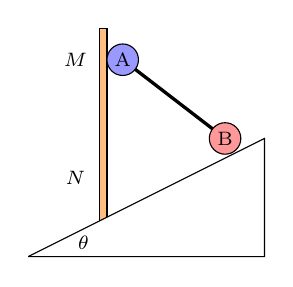
\begin{tikzpicture}[font=\scriptsize]
      \draw[fill=orange!50] (-.1,-.2) rectangle(0,2.4);
      \draw[very thick] (.2,2)--(1.5,1);
      \draw[fill=blue!40] (0.2,2)node{A} circle(.2);
      \draw[fill=red!40] (1.5,1)node{B} circle(.2);
      \filldraw[fill=white] (-1,-.5)--(2,-.5)--(2,1)--(-1,-.5);
      \node at(-.3,-.33){\(\theta\)};
      \node at(-.4,2){\(M\)};
      \node at(-.4,.5){\(N\)};
\end{tikzpicture}
\begin{choices}
    \item \(mg\tan\theta\)
    \item \(\frac{2mg}{\tan\theta}\)
    \item \(\frac{mg}{\tan\theta}\)
    \item \(2mg\tan\theta\)
\end{choices}
\begin{answer}
    D
\end{answer}